\documentclass[11pt,letterpaper]{article}

\usepackage[margin=1in]{geometry}
\usepackage{amsmath,amssymb,amsthm,bm}
\usepackage{booktabs}
\usepackage{enumitem}
\usepackage{xcolor}
\usepackage{graphicx}
\usepackage{tcolorbox}
\usepackage[colorlinks=true,linkcolor=blue!55!black,urlcolor=blue!55!black,citecolor=blue!55!black]{hyperref}

\graphicspath{{figs/}{notes/figs/}}

% Plain-language call-out box for readers new to quantum spin ice.
\newtcolorbox{intuition}[1][]{colback=blue!4,colframe=blue!35!black,
  boxrule=0.5pt,arc=2pt,left=6pt,right=6pt,top=4pt,bottom=4pt,
  fonttitle=\bfseries,title={In plain language},#1}

\newcommand{\Jzz}{J_{zz}}
\newcommand{\Jpm}{J_{\pm}}
\newcommand{\Heff}{H_{\mathrm{eff}}}
\newcommand{\Hclean}{H_{\mathrm{clean}}}
\newcommand{\gfour}{g_4}
\newcommand{\ghex}{g_{\mathrm{hex}}}
\newcommand{\bA}{\bm A}
\newcommand{\bd}{\bm d}
\newcommand{\bn}{\bm n}
\newcommand{\bN}{\bm N}
\newcommand{\bL}{\bm L}
\newcommand{\br}{\bm r}
\newcommand{\bw}{\bm w}
\newcommand{\bq}{\bm q}
\newcommand{\brho}{\bm \rho}
\newcommand{\bdelta}{\bm \delta}
\newcommand{\bDelta}{\bm \Delta}
\newcommand{\bphi}{\bm \phi}
\newcommand{\btheta}{\bm \theta}
\newcommand{\bW}{\bm W}
\newcommand{\Z}{\mathbb Z}
\newcommand{\Tr}{\operatorname{Tr}}
\newcommand{\sgn}{\operatorname{sgn}}
\newcommand{\ice}{\mathcal I}
\newcommand{\cycle}{\mathcal C}
\newcommand{\row}{\mathcal R}
\newcommand{\HB}{H_{\mathrm{band}}}
\newcommand{\Hmic}{H_{\mathrm{mic}}}

\theoremstyle{plain}
\newtheorem{proposition}{Proposition}
\newtheorem{lemma}{Lemma}
\newtheorem{corollary}{Corollary}
\theoremstyle{definition}
\newtheorem{definition}{Definition}
\newtheorem{remark}{Remark}

\title{Pedagogical notes on removing finite-size winding loops in exact
diagonalization of quantum spin ice}
\author{}
\date{\today}

\begin{document}
\maketitle

\begin{abstract}
Exact diagonalization (ED) is an unbiased route to the finite-temperature
physics of the $\pi$-flux quantum spin ice (QSI) regime, where QMC has a
sign problem.  The obstacle is not the usual small-system limitation alone:
periodic pyrochlore clusters contain ice-preserving ring exchanges that
close only by winding around the torus.  The dominant artifact is a
four-site loop generated at order $\Jpm^2$, whereas the physical QSI photon
ring exchange is the contractible six-site hexagon generated at order
$|\Jpm|^3$.  These notes derive this statement, explain why ordinary
boundary-twist averaging does not remove the artifact, and prove the
zero-transport projection criterion
\[
        \bdelta=\brho+\bN\bL=0
\]
for cleaning the ice-manifold effective Hamiltonian.  All numerical tables
quoted below are produced by the standalone script
\texttt{notes/recompute\_finite\_size\_artifact.py}, which rebuilds the
lattice, perturbation theory, projector, and thermodynamics without using
the old project scripts or git history.
\end{abstract}

\tableofcontents

\section{The idea in one page (for readers new to spin ice)}

Before any equations, here is the whole story in words and pictures.

\begin{itemize}
\item \textbf{What the material is.}  ``Quantum spin ice'' (QSI) is a magnet
in which the atomic magnetic moments sit on a lattice of corner-sharing
tetrahedra (the \emph{pyrochlore} lattice).  On every tetrahedron the moments
obey a local rule: two point in and two point out
(Fig.~\ref{fig:ice_rule}).  This is the same counting rule that governs the
proton positions in ordinary water ice, hence the name.  There are
astronomically many ways to satisfy it, so the system has a huge
ground-state degeneracy.

\item \textbf{What makes it ``quantum''.}  A small quantum-mechanical term
lets pairs of neighbouring moments flip.  Acting over and over, these flips
let the system tunnel between different two-in--two-out patterns.  The
smallest tunnelling move that respects the ice rule everywhere is a
\emph{six-spin ring exchange} around a hexagon
(Fig.~\ref{fig:diamond_hexagon} and Fig.~\ref{fig:ring_exchange}).  Remarkably,
the collective dynamics of these ring flips is described by an emergent
\emph{light}: QSI hosts its own artificial photon.  This is what makes the
material exciting, and it is what we want to compute.

\item \textbf{Why the computation is hard.}  We solve the model on a computer
by exact diagonalization (ED), which requires a \emph{finite} block of the
lattice with periodic boundaries---mathematically a doughnut, or
\emph{torus}.  On a torus, some sequences of flips close up not because they
form a real loop in space, but only because they run off one face and come
back on the opposite face (Fig.~\ref{fig:torus_winding}).  The shortest such
``wrap-around'' move involves only \emph{four} spins, and---crucially---it
appears at a lower order in perturbation theory than the physical six-spin
hexagon.  It is a pure artifact of the finite box, yet it is numerically
\emph{larger} than the physics we are after (Fig.~\ref{fig:scale_sep}).

\item \textbf{The symptom.}  Left untreated, this artifact puts the
low-temperature specific-heat peak---one of the cleanest experimental
fingerprints of the emergent photon---in the wrong place, at the artifact
scale $g_4\propto J_\pm^2$ instead of the photon scale
$g_{\mathrm{hex}}\propto|J_\pm|^3$ (Figs.~\ref{fig:ct_twopeak}
and~\ref{fig:specific_heat_all_cases}).

\item \textbf{The cure.}  The physical hexagon closes in real space; the
artifact only closes through the wall of the box.  We give a single
gauge-invariant number, the \emph{transported dipole}
$\bdelta=\brho+\bN\bL$, that is exactly zero for real-space processes and
nonzero for wrap-around ones (Fig.~\ref{fig:real_loops}).  Keeping only the
$\bdelta=0$ processes removes the artifact and leaves the physics untouched.
We also show why the popular fix of ``boundary-twist averaging'' only removes
\emph{half} of the artifact and is therefore not enough
(Fig.~\ref{fig:twist_fail}).
\end{itemize}

The rest of these notes makes each of these statements precise and checks
every number with an independent, from-scratch script.

\section{The physical question}

The QSI Hamiltonian considered here is the nearest-neighbor XXZ model in
local pyrochlore frames,
\begin{equation}
H =
\Jzz\sum_{\langle ij\rangle} S_i^zS_j^z
-\Jpm\sum_{\langle ij\rangle}
\left(S_i^+S_j^-+S_i^-S_j^+\right),
\qquad |\Jpm|\ll \Jzz,\quad \Jzz>0 .
\label{eq:model}
\end{equation}
The Ising part has an extensively degenerate ground manifold: every
tetrahedron has two spins pointing in and two spins pointing out.  This is
the ice manifold $\ice$.

For $\Jpm>0$, the off-diagonal matrix elements in the $S^z$ basis are
non-positive, and standard QMC can be sign-problem-free.  For $\Jpm<0$,
the off-diagonal matrix elements have the opposite sign.  This is the
frustrated $\pi$-flux QSI sector.  It is precisely the sector where ED is
most valuable, because QMC no longer gives an unbiased finite-temperature
benchmark.

The central difficulty is that ED necessarily uses a finite periodic
cluster.  Such a cluster is a torus.  On a torus, paths can close by
periodic identification even when they do not close in real space.  Some of
these winding paths preserve the ice rule and therefore appear directly in
the low-energy gauge Hamiltonian.  The shortest such processes on the
standard 16-site cubic and 32-site FCC clusters are four-site loops.  They
are not physical bulk plaquettes.  Nevertheless, they strongly affect the
low-temperature specific heat and the low-frequency $S^{zz}(\bq,\omega)$.

\section{Ice variables and the energy cost of defects}

\begin{figure}[htbp]
\centering
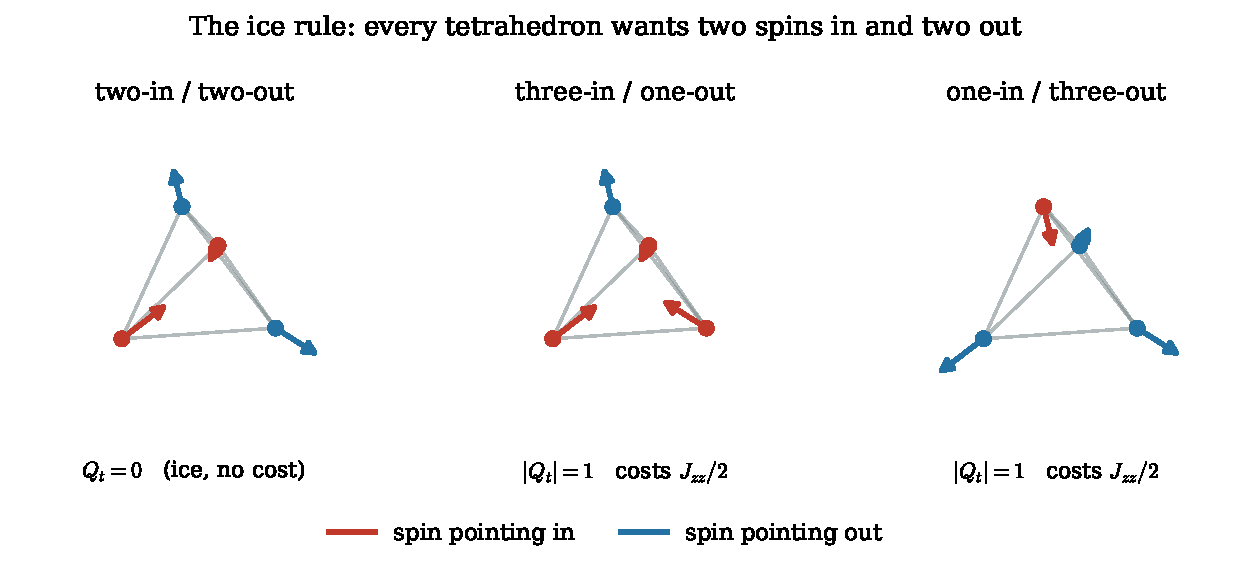
\includegraphics[width=0.95\textwidth]{fig_ice_rule.pdf}
\caption{\textbf{The ice rule.}  Each spin lives on a corner of a
tetrahedron and points either into the tetrahedron (red) or out of it
(blue).  \emph{Left:} the low-energy ``ice'' configuration has two in and two
out, so the net Ising charge $Q_t=\sum_{i\in t}S_i^z$ vanishes and the
tetrahedron pays no energy.  \emph{Middle, right:} tipping one spin makes the
tetrahedron three-in--one-out or one-in--three-out, with $|Q_t|=1$; by
Eq.~\eqref{eq:tet_energy} this costs $\Jzz/2$.  These charged tetrahedra are
the ``spinons'' of quantum spin ice.}
\label{fig:ice_rule}
\end{figure}

For a tetrahedron $t$, define the Ising charge
\begin{equation}
Q_t=\sum_{i\in t} S_i^z .
\end{equation}
For spin $1/2$, $S_i^z=\pm 1/2$.  The Ising energy on one tetrahedron is
\begin{equation}
\sum_{\langle ij\rangle\in t} S_i^zS_j^z
=\frac12\left[\left(\sum_{i\in t}S_i^z\right)^2-\sum_{i\in t}(S_i^z)^2\right]
=\frac12 Q_t^2-\frac12 .
\label{eq:tet_energy}
\end{equation}
Thus, up to a constant,
\begin{equation}
H_0=\frac{\Jzz}{2}\sum_t Q_t^2 .
\label{eq:charge_h0}
\end{equation}
The ice rule is $Q_t=0$ on every tetrahedron.  A $3$-in--$1$-out or
$1$-in--$3$-out tetrahedron has $|Q_t|=1$ and costs $\Jzz/2$ relative to an
ice tetrahedron.

Now act with a transverse exchange
\[
S_i^+S_j^-+S_i^-S_j^+
\]
on an antiparallel nearest-neighbor pair.  The two sites $i$ and $j$ lie on
one common tetrahedron, where exchanging an up and a down spin preserves
$Q_t=0$.  Each site also belongs to one other tetrahedron.  Those two
neighboring tetrahedra become charged, each costing $\Jzz/2$.  Therefore a
single nearest-neighbor exchange out of the ice manifold creates two
defects with total cost
\begin{equation}
\Delta_{\mathrm{1hop}}=\Jzz .
\label{eq:one_hop_cost}
\end{equation}
This simple denominator is the origin of the perturbative scales below.

\begin{intuition}
A single spin flip is like pushing one domino: it necessarily unbalances
the two tetrahedra that share that spin, creating a pair of oppositely
charged defects that together cost $\Jzz$.  To get back into the ice manifold
you must flip more spins so that every tetrahedron is balanced again.  The
cheapest way to do that around a closed path is what the next sections count.
\end{intuition}

\section{Degenerate perturbation theory in the ice manifold}

Let $P$ be the projector onto the ice manifold and $Q=1-P$.  Write
\[
H=H_0+V,\qquad
V=-\Jpm\sum_{\langle ij\rangle}
\left(S_i^+S_j^-+S_i^-S_j^+\right).
\]
The ice energy is shifted to zero.  The non-ice resolvent is
\begin{equation}
R=Q\frac{1}{E_{\ice}-H_0}Q=-QH_0^{-1}Q .
\end{equation}
Because a single exchange leaves the ice manifold, $PVP=0$.  The first
nonzero terms are therefore
\begin{align}
\Heff^{(2)} &= PVRVP, \label{eq:heff2}\\
\Heff^{(3)} &= PVRVRVP. \label{eq:heff3}
\end{align}
For a path $s\to m_1\to \cdots \to t$, its contribution has the form
\begin{equation}
\langle t|\Heff^{(k)}|s\rangle
=
\sum_{\mathrm{paths}}
\frac{\langle t|V|m_{k-1}\rangle\cdots
\langle m_1|V|s\rangle}
{(E_\ice-E_{m_1})\cdots(E_\ice-E_{m_{k-1}})} .
\label{eq:path_pt}
\end{equation}
Each matrix element of $V$ contributes a factor $-\Jpm$, and each
intermediate energy denominator is negative.

\begin{remark}
The standalone recomputation stores each perturbative process as a row
\[
        r=(s,t,\bN,c,k),
\]
meaning that the row connects ice states $s$ and $t$, appears at order $k$,
has coefficient $c$ when $\Jpm=1$, and has accumulated periodic image
transport $\bN$.  At physical coupling, the row contributes
$c\Jpm^k|t\rangle\langle s|$.
\end{remark}

\section{Why the physical QSI ring exchange is a hexagon}

\begin{figure}[htbp]
\centering
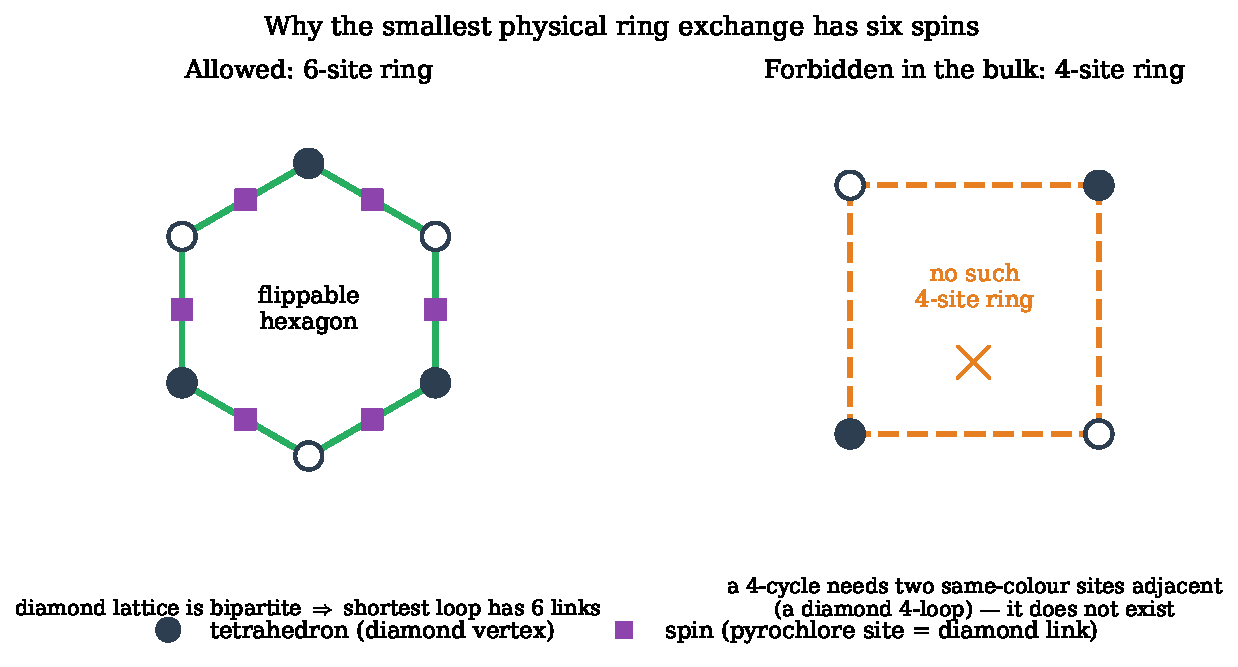
\includegraphics[width=0.92\textwidth]{fig_diamond_hexagon.pdf}
\caption{\textbf{The smallest real ring exchange has six spins.}  Each
tetrahedron is a vertex of the diamond lattice (circles); each spin is a link
of that lattice (squares).  A ring exchange must flip an alternating chain of
spins around a closed loop of tetrahedra.  \emph{Left:} the diamond lattice is
bipartite (two colours, links only join different colours), so its shortest
loop uses six links---a six-spin hexagon.  \emph{Right:} a four-spin ring
would require a four-loop on the diamond lattice, which would need two
same-colour vertices to be adjacent; no such loop exists in the bulk.  This is
the geometric reason a contractible four-site ice loop is impossible.}
\label{fig:diamond_hexagon}
\end{figure}

The pyrochlore lattice is the line graph of the diamond lattice: a
pyrochlore site corresponds to a diamond bond, and a pyrochlore
tetrahedron corresponds to a diamond vertex.  An ice configuration assigns
a divergence-free electric field to diamond bonds.  A ring exchange in the
ice manifold must flip an alternating set of spins around a closed path so
that the divergence at every touched diamond vertex remains zero.

\begin{lemma}[Shortest contractible ice loop]
The shortest nontrivial contractible ice-preserving ring exchange on the
infinite pyrochlore lattice is a six-site hexagon.
\end{lemma}

\begin{proof}
An ice-preserving loop must enter and leave every touched tetrahedron, so
on the diamond lattice it corresponds to a closed non-backtracking loop.
The diamond lattice is bipartite and has no triangles.  It also has no
four-cycles; its elementary loops are length six.  Therefore the shortest
contractible closed diamond loop has length six.  Mapping back to the
pyrochlore line graph gives a six-site pyrochlore hexagon.  A triangle of
the pyrochlore graph lies inside one tetrahedron and is not an alternating
ice ring.  A contractible four-site ice ring would map to a diamond
four-cycle, which does not exist.
\end{proof}

\subsection{Third-order hexagon amplitude}

\begin{figure}[htbp]
\centering
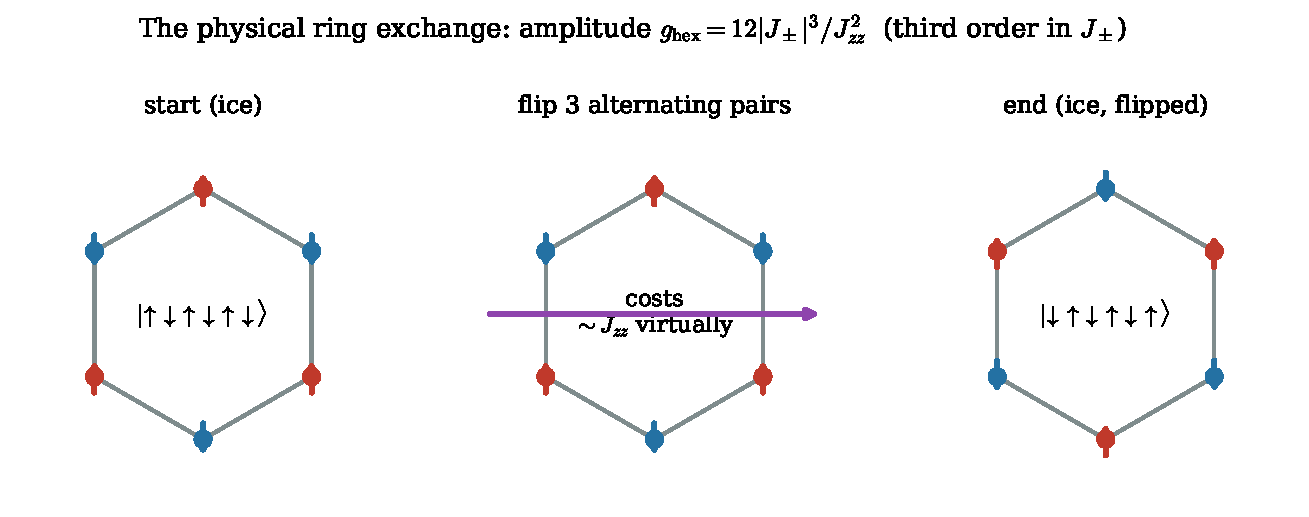
\includegraphics[width=0.95\textwidth]{fig_ring_exchange.pdf}
\caption{\textbf{The physical ring exchange (the emergent-photon move).}
Starting from an alternating up/down pattern on a hexagon, flipping all three
alternating pairs turns each up into a down and vice versa, returning to the
ice manifold.  Because the intermediate steps leave the ice manifold, the
amplitude is third order in $J_\pm$, with magnitude
$g_{\mathrm{hex}}=12|J_\pm|^3/J_{zz}^2$.  The coherent superposition of these
ring flips across the lattice is the artificial photon of quantum spin ice.}
\label{fig:ring_exchange}
\end{figure}

Consider a flippable hexagon with alternating spins.  To move from one ice
configuration to the flipped configuration, one must exchange three
alternating nearest-neighbor pairs.  After the first exchange the system
has two charged tetrahedra and costs $\Jzz$.  After the second exchange it
still has a pair of charged tetrahedra and costs $\Jzz$.  Thus each
ordering gives a denominator $\Jzz^2$.

For one orientation there are $3!$ orderings.  Including the Hermitian
conjugate orientation gives the conventional ring term
\begin{equation}
\Heff^{\mathrm{hex}}
=-\ghex\sum_{\mathrm{hex}}
\left(
S_1^+S_2^-S_3^+S_4^-S_5^+S_6^-+\mathrm{h.c.}
\right),
\end{equation}
with magnitude
\begin{equation}
\boxed{
\ghex=\frac{12|\Jpm|^3}{\Jzz^2}.
}
\label{eq:ghex}
\end{equation}
The sign of the effective ring term follows $\sgn(\Jpm^3)$.  This sign is
what distinguishes the $0$-flux and $\pi$-flux gauge sectors.

\section{Why a four-site loop is a finite-size artifact}

\begin{figure}[htbp]
\centering
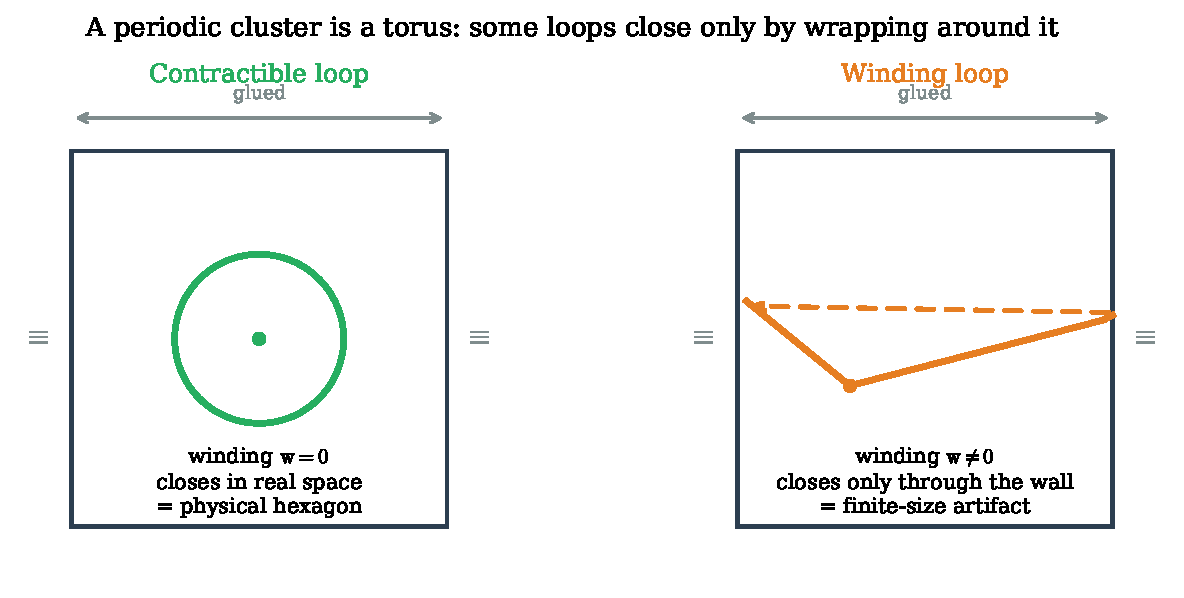
\includegraphics[width=0.9\textwidth]{fig_torus_winding.pdf}
\caption{\textbf{A periodic cluster is a torus.}  Opposite walls of the
simulation box are identified (glued), so the box is topologically a
doughnut.  \emph{Left:} a loop that closes inside the box has winding
$\bw=0$; it is a genuine real-space process such as the physical hexagon.
\emph{Right:} a path can also close by leaving one wall and re-entering the
opposite wall.  Its winding $\bw\neq0$; it exists \emph{only} because of the
periodic gluing and has no counterpart in the infinite lattice.}
\label{fig:torus_winding}
\end{figure}

A periodic cluster is not $\mathbb R^3$; it is the flat torus
\begin{equation}
T^3=\mathbb R^3/(\Z^3\bL) ,
\end{equation}
where we use row vectors and the rows of $\bL$ are the three cluster
translation vectors.  Thus $\bm m\bL$, with $\bm m\in\Z^3$, is a periodic
translation.  For the cubic $L_1\times L_2\times L_3$ cluster,
\[
\bL=\begin{pmatrix}
L_1&0&0\\
0&L_2&0\\
0&0&L_3
\end{pmatrix}.
\]
For the FCC primitive cluster, the rows are
$L_1(\tfrac12,\tfrac12,0)$, $L_2(\tfrac12,0,\tfrac12)$, and
$L_3(0,\tfrac12,\tfrac12)$.  All coordinates in this note are measured in
conventional cubic-cell units.  The pyrochlore basis sites lie on the
quarter-lattice,
\[
\br_i\in \frac14\Z^3,
\]
which is the reason factors of $4$ appear below.

A bond
from site $i$ to site $j$ is represented by a minimum-image displacement
\begin{equation}
\bd_{ij}=\br_j-\br_i-\bn_{ij}\bL,
\qquad \bn_{ij}\in\Z^3 .
\end{equation}
For a closed path $\cycle$ on the periodic graph, define its winding vector
\begin{equation}
\bw_\cycle=\sum_{(ij)\in\cycle}\bn_{ij}.
\label{eq:winding}
\end{equation}
If $\bw_\cycle=0$, the lifted path closes in real space and is
contractible.  If $\bw_\cycle\ne0$, the path closes only because opposite
faces of the cluster have been identified.

\begin{proposition}[No physical four-loop]
Every ice-preserving four-cycle on the standard $1\times1\times1$ cubic
and $2\times2\times2$ FCC pyrochlore clusters is a winding torus loop, not
a contractible bulk process.
\end{proposition}

\begin{proof}
The geometric lemma above rules out a contractible four-site ice loop on
the infinite pyrochlore lattice.  Therefore any four-site ice loop observed
on a periodic cluster must use the periodic identification.  Equivalently,
its lift to $\mathbb R^3$ fails to close and has nonzero winding
$\bw_\cycle$.  The explicit independent enumeration below verifies this
for the two clusters used in the ED calculation.
\end{proof}

\subsection{Second-order four-loop amplitude}

\begin{figure}[htbp]
\centering
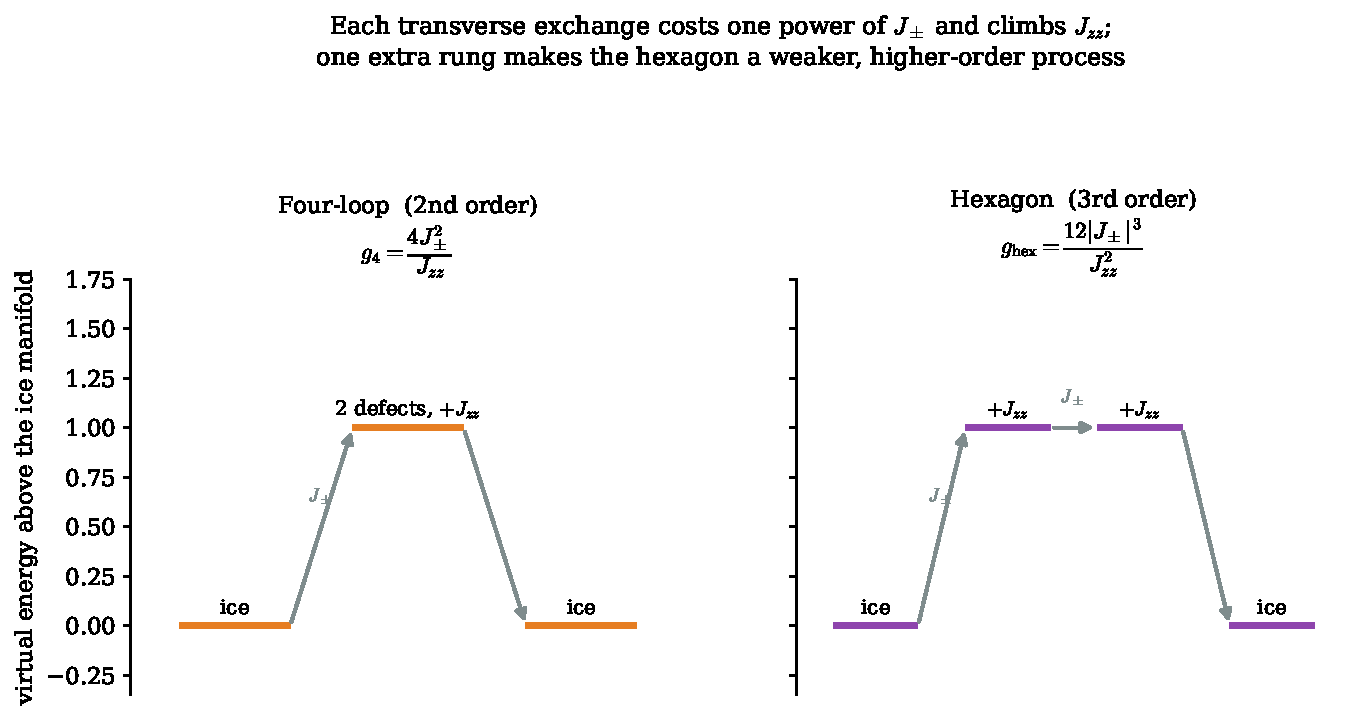
\includegraphics[width=0.95\textwidth]{fig_pt_ladder.pdf}
\caption{\textbf{Counting the powers of $J_\pm$.}  Every transverse exchange
adds one factor of $J_\pm$ and pushes the system one virtual step above the
ice manifold, where it costs $\sim\Jzz$.  \emph{Left:} the winding four-loop
returns to the ice manifold after just two exchanges (one intermediate
tetrahedron pair), giving $g_4=4J_\pm^2/\Jzz$.  \emph{Right:} the hexagon
needs three exchanges (two intermediate steps), giving the weaker,
higher-order $g_{\mathrm{hex}}=12|J_\pm|^3/\Jzz^2$.  The extra rung is the
entire reason the artifact is parametrically larger at small $J_\pm$.}
\label{fig:pt_ladder}
\end{figure}

A winding four-loop has four alternating sites and can be flipped by two
nearest-neighbor exchanges.  The two exchanged bonds form a perfect
matching of the four sites.  There are two matchings, and for each matching
there are two time orderings.  Each path has one intermediate state with
energy cost $\Jzz$.  Thus the magnitude of the second-order matrix element
is
\begin{equation}
4\frac{\Jpm^2}{\Jzz}.
\end{equation}
In the ring-exchange convention used here,
\begin{equation}
\boxed{
\gfour=\frac{4\Jpm^2}{\Jzz}.
}
\label{eq:g4}
\end{equation}
The sign is convention dependent, but the scale is not.

The scale separation is
\begin{equation}
\boxed{
\frac{\gfour}{\ghex}
=
\frac{4\Jpm^2/\Jzz}{12|\Jpm|^3/\Jzz^2}
=
\frac{\Jzz}{3|\Jpm|}.
}
\label{eq:scale_separation}
\end{equation}
Thus the artifact becomes more severe precisely in the perturbative regime
where the QSI description is best controlled.

\begin{figure}[htbp]
\centering
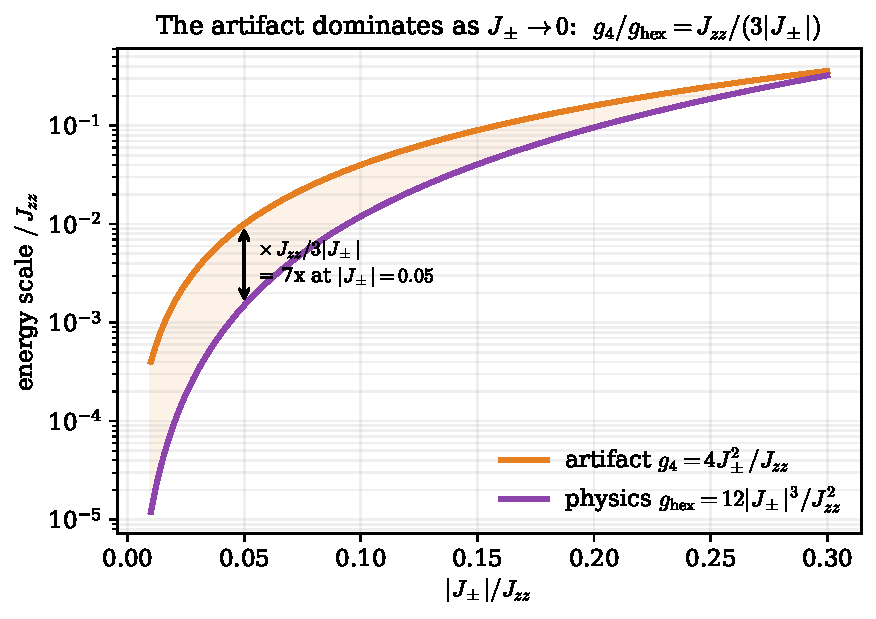
\includegraphics[width=0.62\textwidth]{fig_scale_sep.pdf}
\caption{\textbf{The artifact dominates exactly where we want to work.}  The
finite-size four-loop scale $g_4$ (orange) and the physical photon scale
$g_{\mathrm{hex}}$ (purple) both vanish as $J_\pm\to0$, but their ratio
$g_4/g_{\mathrm{hex}}=\Jzz/(3|J_\pm|)$ \emph{grows}.  At the representative
value $|J_\pm|=0.05\,\Jzz$ the artifact is already $\sim7\times$ larger than
the physics it would otherwise swamp.}
\label{fig:scale_sep}
\end{figure}

\section{Independent numerical verification}

The script
\[
\texttt{notes/recompute\_finite\_size\_artifact.py}
\]
does not import the old \texttt{twist\_qsi\_demo/scripts} code and does not
inspect git history.  It independently:
\begin{enumerate}[label=(\roman*)]
\item builds the pyrochlore positions, nearest-neighbor graph, tetrahedra,
and periodic image vectors;
\item enumerates all two-in--two-out ice states;
\item enumerates ice-preserving four-cycles and hexagons;
\item constructs $H_2=PVRVP$ and $H_3=PVRVRVP$ from path sums;
\item applies either no projector or the zero-transport projector derived
below;
\item diagonalizes the resulting ice-manifold Hamiltonian and computes
$C(T)$.
\end{enumerate}
The raw output is saved in
\texttt{notes/recomputed\_finite\_size\_artifact.json}.

\subsection{Geometry census}

\begin{center}
\begin{tabular}{lrrrrr}
\toprule
cluster & sites & ice states & 4-cycles & contractible 4-cycles
& contractible hexagons \\
\midrule
cubic $1\times1\times1$ & 16 & 90 & 36 & 0 & 16 \\
FCC $2\times2\times2$ & 32 & 2970 & 24 & 0 & 32 \\
\bottomrule
\end{tabular}
\end{center}

The same enumeration finds 48 wrapping hexagons on the 16-site cluster and
96 wrapping hexagons on the 32-site cluster.  Those are also finite-size
torus processes, but they appear at the same order as the physical
hexagons.  The four-loops are the dominant contamination because they
appear one order earlier.

\section{Why the low-temperature specific heat peak is displaced}

For an exact spectrum $\{E_n\}$, shifted so $E_0=0$,
\begin{equation}
Z(T)=\sum_n e^{-E_n/T},\qquad
\langle E^p\rangle_T=\frac{1}{Z}\sum_n E_n^p e^{-E_n/T},
\end{equation}
and
\begin{equation}
C(T)=\frac{\langle E^2\rangle_T-\langle E\rangle_T^2}{T^2}.
\label{eq:specific_heat}
\end{equation}
For a two-level system with splitting $\Delta$,
\begin{equation}
C_{\mathrm{2lev}}(T)
=\frac{(\Delta/T)^2 e^{-\Delta/T}}
{\left(1+e^{-\Delta/T}\right)^2},
\end{equation}
whose maximum is at $T=O(\Delta)$.  A many-level finite cluster has a more
complicated spectrum, but the lower peak still tracks the dominant
low-energy splitting scale in the ice manifold.

Therefore:
\begin{align}
T_{\mathrm{peak}}^{\mathrm{bare}} &\sim \gfour\propto \Jpm^2,
\qquad\text{if winding four-loops are present},\\
T_{\mathrm{peak}}^{\mathrm{clean}} &\sim \ghex\propto |\Jpm|^3,
\qquad\text{after winding transport is removed}.
\end{align}

\begin{figure}[htbp]
\centering
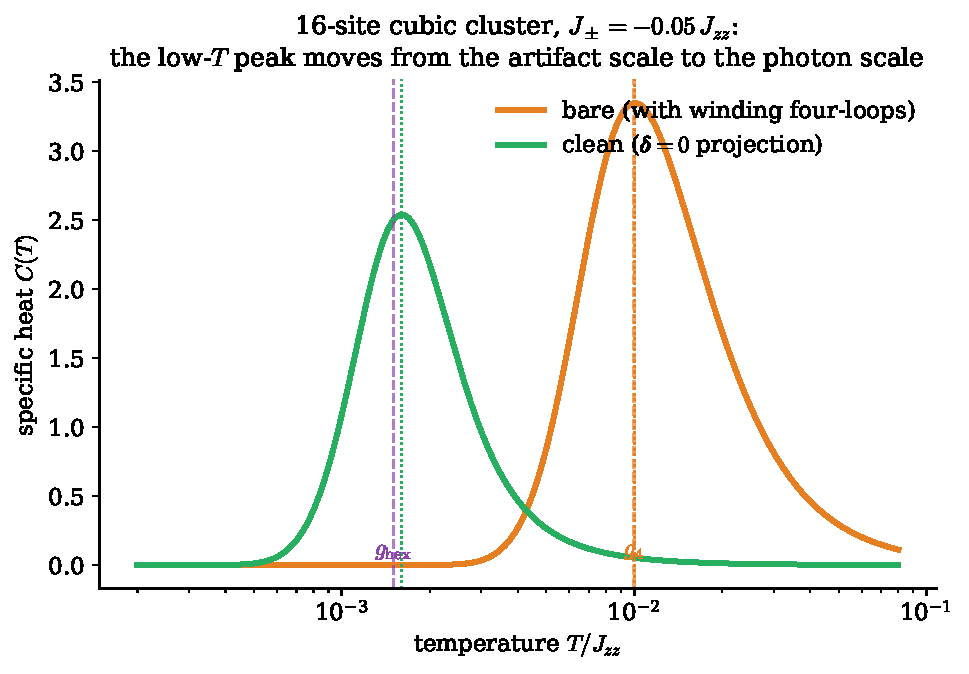
\includegraphics[width=0.66\textwidth]{fig_ct_twopeak.pdf}
\caption{\textbf{The low-temperature specific-heat peak is displaced by the
artifact.}  Exact specific heat of the $16$-site cubic ice-manifold
Hamiltonian at $J_\pm=-0.05\,\Jzz$.  The bare cluster (orange) peaks at the
artifact scale $g_4$; after the $\bdelta=0$ projection (green) the peak drops
onto the physical photon scale $g_{\mathrm{hex}}$---nearly an order of
magnitude lower in temperature.  Since the specific heat is a nonlinear
function of the spectrum, this shift cannot be undone by averaging $C(T)$
after the fact (Sec.~\ref{sec:operator-level}).}
\label{fig:ct_twopeak}
\end{figure}

\begin{figure}[htbp]
\centering
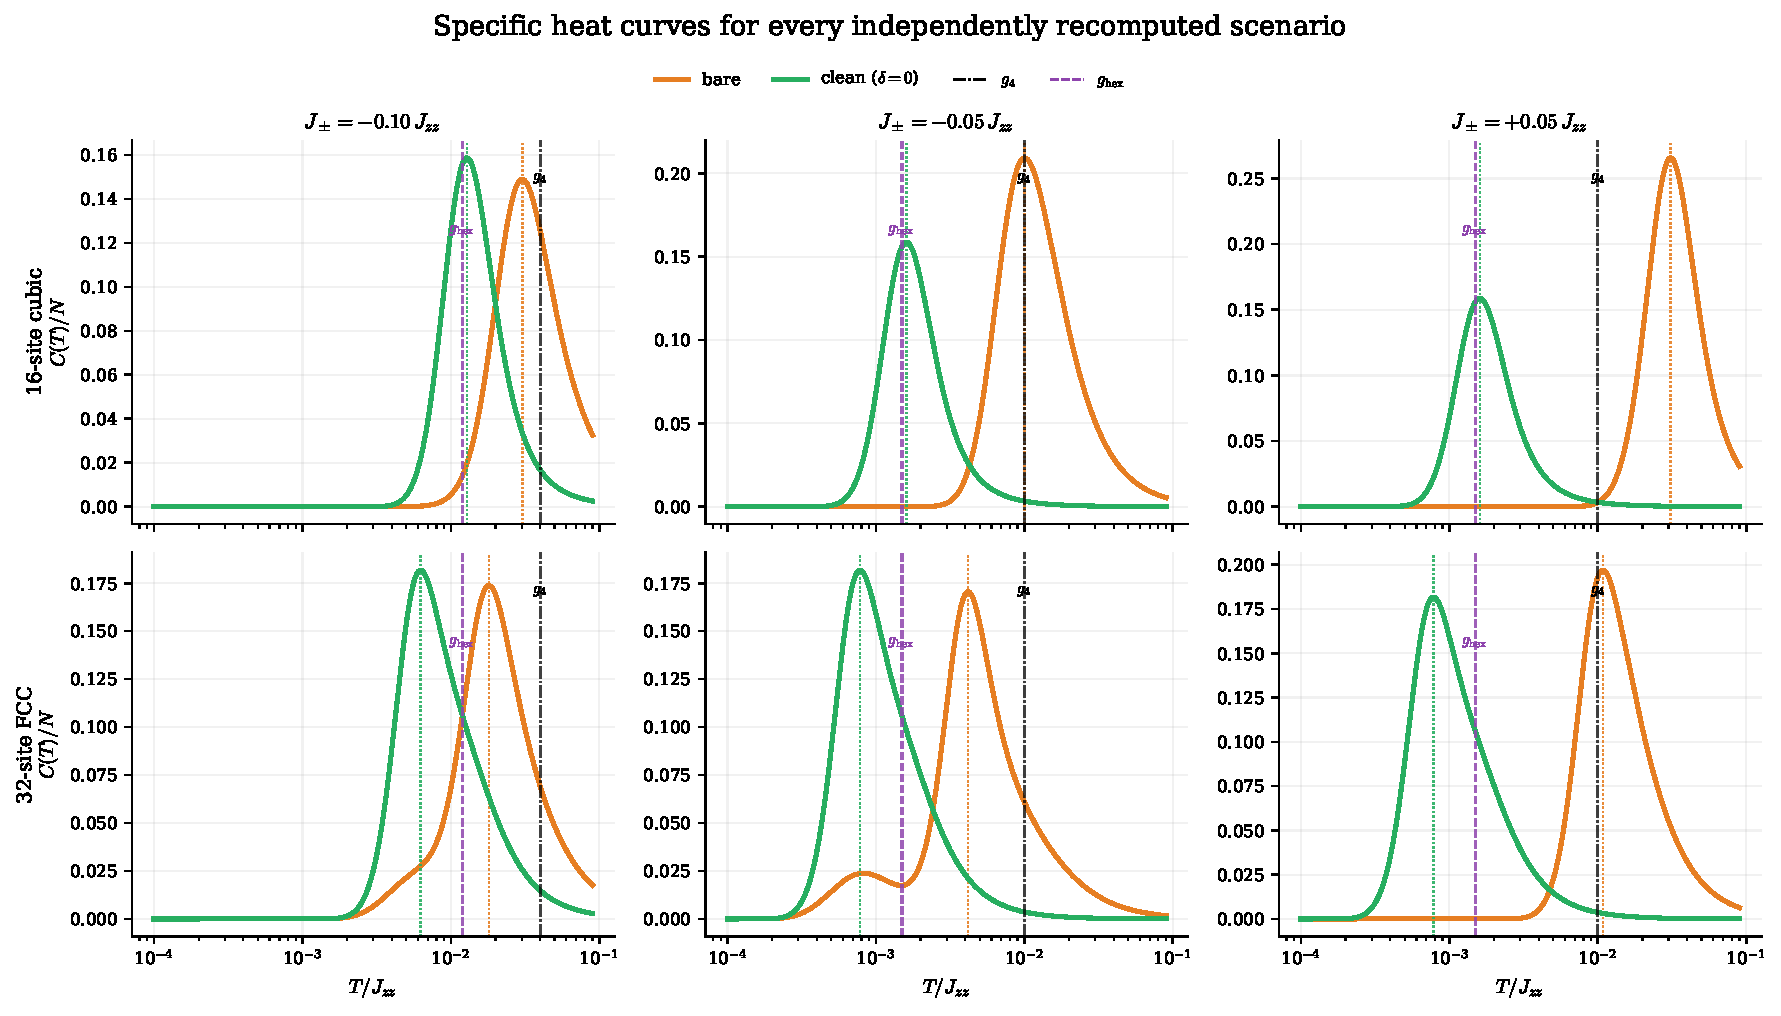
\includegraphics[width=\textwidth]{fig_specific_heat_all_cases.pdf}
\caption{\textbf{Specific heat as a function of temperature for all
independently recomputed scenarios.}  Each panel shows the exact
ice-manifold specific heat per site, $C(T)/N$, from the standalone
Schrieffer--Wolff calculation.  The columns are the three computed
couplings, and the rows are the two ED clusters.  Orange is the bare
periodic effective Hamiltonian; green is the zero-transport
$(\bdelta=0)$ Hamiltonian.  Dotted orange/green vertical lines mark the
actual peak positions of the two curves, the black dash-dot line marks
$g_4$, and the purple dashed line marks $g_{\mathrm{hex}}$.  The full
curves show the same conclusion as the peak table: removing transported
winding processes shifts the low-temperature feature from the finite-size
scale toward the photon scale.}
\label{fig:specific_heat_all_cases}
\end{figure}

The independent calculation gives the following representative peaks:
\begin{center}
\begin{tabular}{llrrr}
\toprule
cluster & Hamiltonian & $\Jpm$ & $T_{\mathrm{peak}}$ &
scale diagnostic \\
\midrule
cubic $N=16$ & bare & $-0.05$ & 0.010056 &
$T_{\mathrm{peak}}/g_4=1.01$ \\
cubic $N=16$ & clean & $-0.05$ & 0.001604 &
$T_{\mathrm{peak}}/g_{\mathrm{hex}}=1.07$ \\
FCC $N=32$ & bare & $-0.05$ & 0.004180 &
$T_{\mathrm{peak}}/g_{\mathrm{hex}}=2.79$ \\
FCC $N=32$ & clean & $-0.05$ & 0.000782 &
$T_{\mathrm{peak}}/g_{\mathrm{hex}}=0.52$ \\
FCC $N=32$ & bare & $-0.10$ & 0.018053 &
$T_{\mathrm{peak}}/g_{\mathrm{hex}}=1.50$ \\
FCC $N=32$ & clean & $-0.10$ & 0.006252 &
$T_{\mathrm{peak}}/g_{\mathrm{hex}}=0.52$ \\
\bottomrule
\end{tabular}
\end{center}
For the 16-site cluster at $\Jpm=-0.05$, $g_4=4(0.05)^2=0.010$ and
$g_{\mathrm{hex}}=12(0.05)^3=0.0015$, so the scale identification is
especially transparent.

\begin{figure}[htbp]
\centering
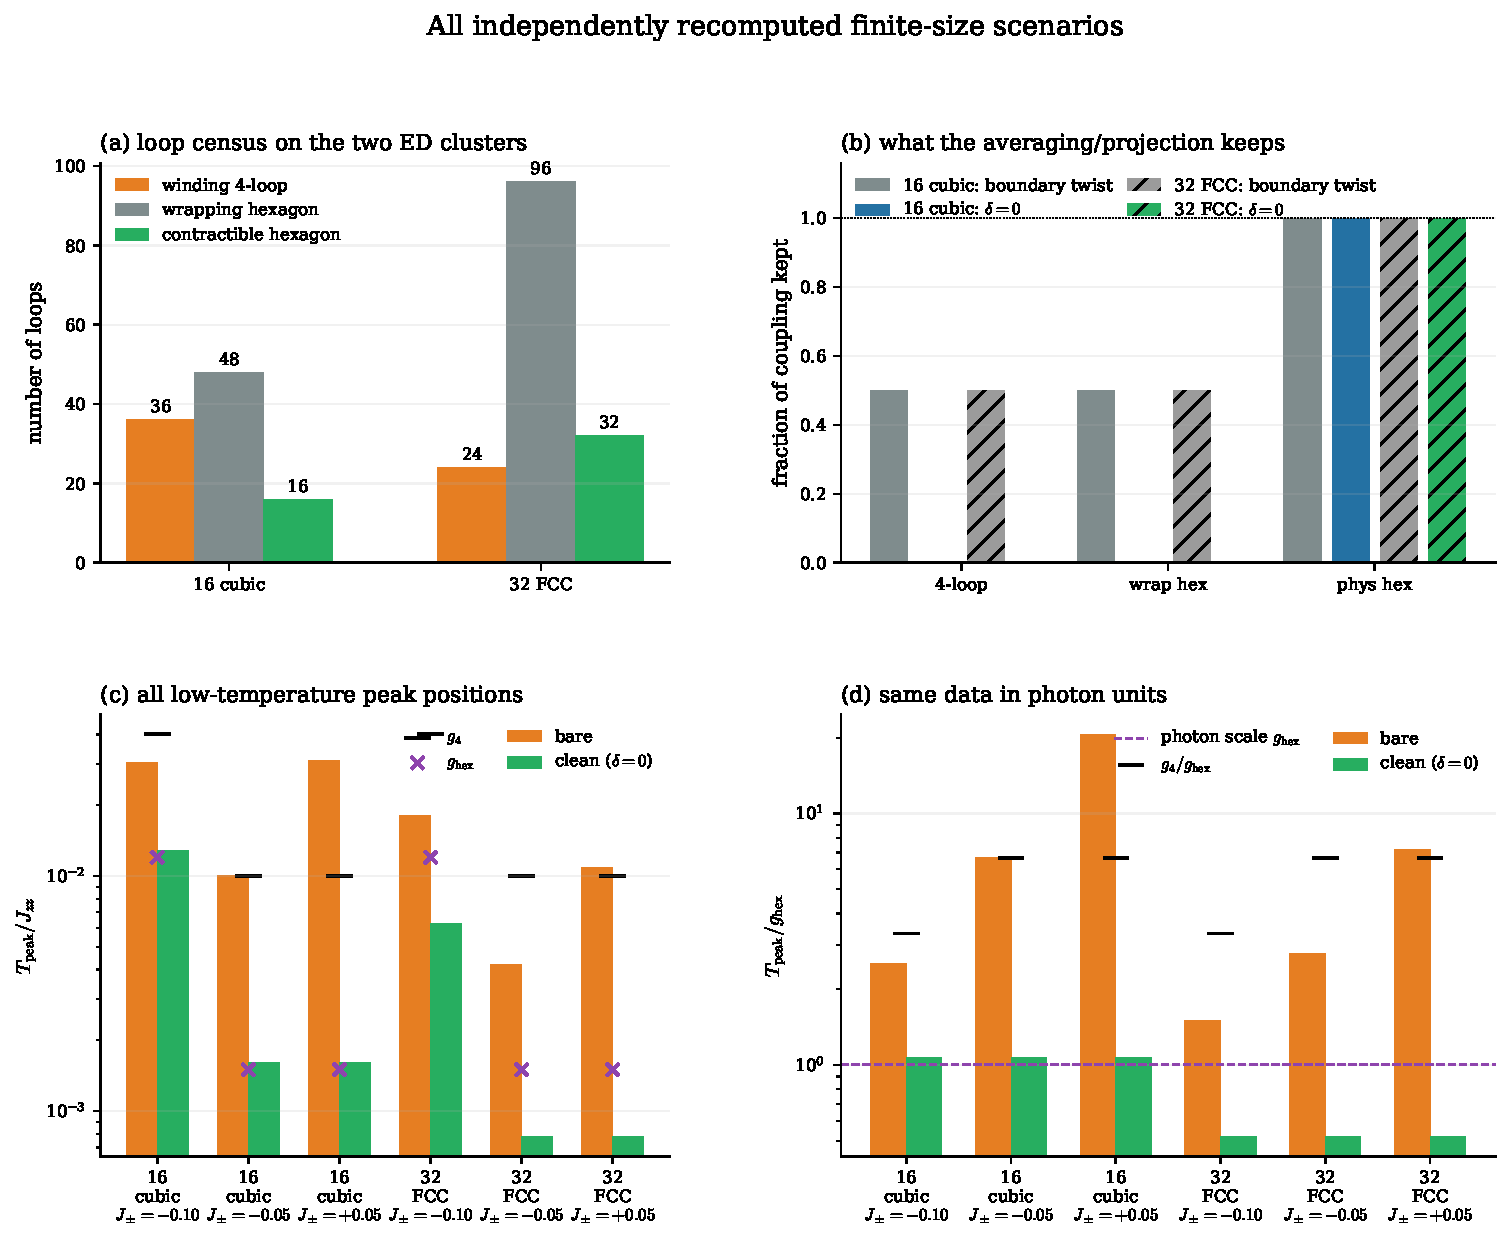
\includegraphics[width=\textwidth]{fig_all_scenarios.pdf}
\caption{\textbf{All independently recomputed finite-size scenarios in one
place.}  \emph{(a)} The two ED clusters both contain winding four-loops
and wrapping hexagons in addition to the physical contractible hexagons.
\emph{(b)} Boundary-twist averaging keeps half of each winding channel on
both clusters, while the zero-transport projector removes them and keeps
the physical hexagon.  \emph{(c)} The low-temperature peak positions for
all computed clusters, flux signs, and projection choices.  Black ticks
mark $g_4$ and purple crosses mark $g_{\mathrm{hex}}$.  \emph{(d)} The same
peak data in photon units.  The cleaned spectra stay at an order-one
multiple of $g_{\mathrm{hex}}$, while the bare spectra are pushed upward by
the winding-loop contamination.}
\label{fig:all_scenarios}
\end{figure}

\section{Why ordinary boundary-twist averaging fails}

Boundary twists are often used to reduce finite-size effects.  Put phases
only on boundary-crossing bonds.  If a virtual path accumulates image
transport $\bN$, its row coefficient becomes
\begin{equation}
c_r(\bphi)=c_r e^{-i\bN_r\cdot\bphi}.
\end{equation}
The eight-corner average over $\phi_a\in\{0,\pi\}$ gives
\begin{equation}
\frac18\sum_{\phi_a=0,\pi}e^{-i\bN\cdot\bphi}
=\prod_{a=1}^3\frac{1+(-1)^{N_a}}{2}.
\label{eq:corner_kernel}
\end{equation}
This keeps rows with even $\bN$.

The subtle point is that the geometric ring exchange is not a single path.
It is a sum over virtual paths.  A winding four-loop has multiple
matchings and time orderings.  Some paths cross the boundary, while other
paths implementing the same geometric flip can have $\bN=0$ in the
boundary gauge.  The corner average therefore kills only part of the
coefficient.

\begin{figure}[htbp]
\centering
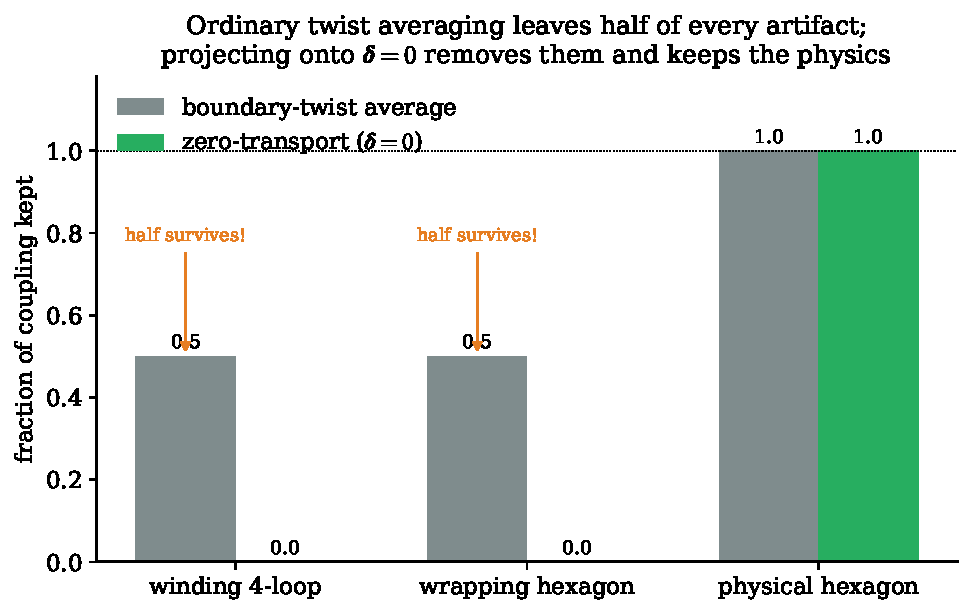
\includegraphics[width=0.66\textwidth]{fig_twist_fail.pdf}
\caption{\textbf{Boundary-twist averaging is not enough.}  Fraction of each
geometric channel's coupling that survives on the $16$-site cubic cluster.
Ordinary boundary-twist (corner) averaging (grey) leaves \emph{half} of every
winding artifact---because the ring exchange is a sum over virtual paths and
some of those paths do not cross the boundary in the chosen gauge.  The
gauge-invariant $\bdelta=0$ projection (green) removes the winding four-loop
and wrapping hexagon completely while keeping the physical hexagon at full
strength.}
\label{fig:twist_fail}
\end{figure}

The standalone recomputation classifies the off-diagonal rows by geometric
channel and gives:
\begin{center}
\begin{tabular}{lccc}
\toprule
channel & corner average kept & $N=0$ kept & zero-transport kept \\
\midrule
4-loop, cubic $N=16$ & 0.5 & 0.5 & 0 \\
wrapping hexagon, cubic $N=16$ & 0.5 & 0.5 & 0 \\
contractible hexagon, cubic $N=16$ & 1 & 1 & 1 \\
4-loop, FCC $N=32$ & 0.5 & 0.5 & 0 \\
wrapping hexagon, FCC $N=32$ & 0.5 & 0.5 & 0 \\
contractible hexagon, FCC $N=32$ & 1 & 1 & 1 \\
\bottomrule
\end{tabular}
\end{center}
Thus ordinary boundary-twist averaging reduces the winding artifact but
does not remove it.

\section{The transported dipole and the zero-transport theorem}
\label{sec:transported-dipole}

The correct object is not the boundary-crossing count of one chosen gauge.
It is the gauge-invariant net displacement transported by the effective
operator.

\begin{definition}[Home-cell dipole]
For a perturbative row connecting ice states $s$ and $t$, define
\[
R_+(t,s)=\{i:S_i^z(t)-S_i^z(s)>0\},\qquad
R_-(t,s)=\{j:S_j^z(t)-S_j^z(s)<0\}.
\]
The set $R_+$ contains spins raised by the effective process; $R_-$ contains
spins lowered by the effective process.  The home-cell dipole is
\begin{equation}
\brho_{t,s}=\sum_{i\in R_+(t,s)}\br_i-\sum_{j\in R_-(t,s)}\br_j .
\label{eq:rho_def}
\end{equation}
\end{definition}

\begin{definition}[Transported dipole]
Let $\bN_r\in\Z^3$ be the accumulated image vector of the virtual path.  In row
vector convention, $\bN_r\bL$ is the net periodic translation needed when the
path is lifted from the torus back to the covering space $\mathbb R^3$.  The
transported dipole is
\begin{equation}
\boxed{
\bdelta_r=\brho_{t,s}+\bN_r\bL .
}
\label{eq:delta_def}
\end{equation}
\end{definition}

The formula is easiest to understand for one microscopic hop.  The operator
$S_i^+S_j^-$ raises site $i$ and lowers site $j$, so its home-cell dipole is
$\br_i-\br_j$.  If the nearest-neighbor bond was represented using the periodic
image vector $\bn_{ij}$, then the lifted displacement of the spin transfer is
\[
\br_i-\br_j+\bn_{ij}\bL=-\bd_{ij}.
\]
The many-step perturbative row adds these lifted increments.  Thus
$\bdelta_r$ is not a new dynamical charge.  It is the net real-space
displacement carried by the virtual spin transfers after the periodic images
have been undone.

For the order-$\Jpm^2$ and order-$\Jpm^3$ ice-manifold rows explicitly
enumerated below, the possible transported dipoles are actually coarser than
the microscopic quarter-lattice: their components lie in $\frac12\Z$.  In other
words, the computed $\bDelta=4\bdelta$ components are always even.  This is a
property of the ice-preserving processes at these orders, not of a single
nearest-neighbor hop.  A single microscopic transverse hop still carries a
quarter-lattice displacement, so the full microscopic source field is most
naturally written with $4\bd_{ij}$.

\begin{figure}[htbp]
\centering
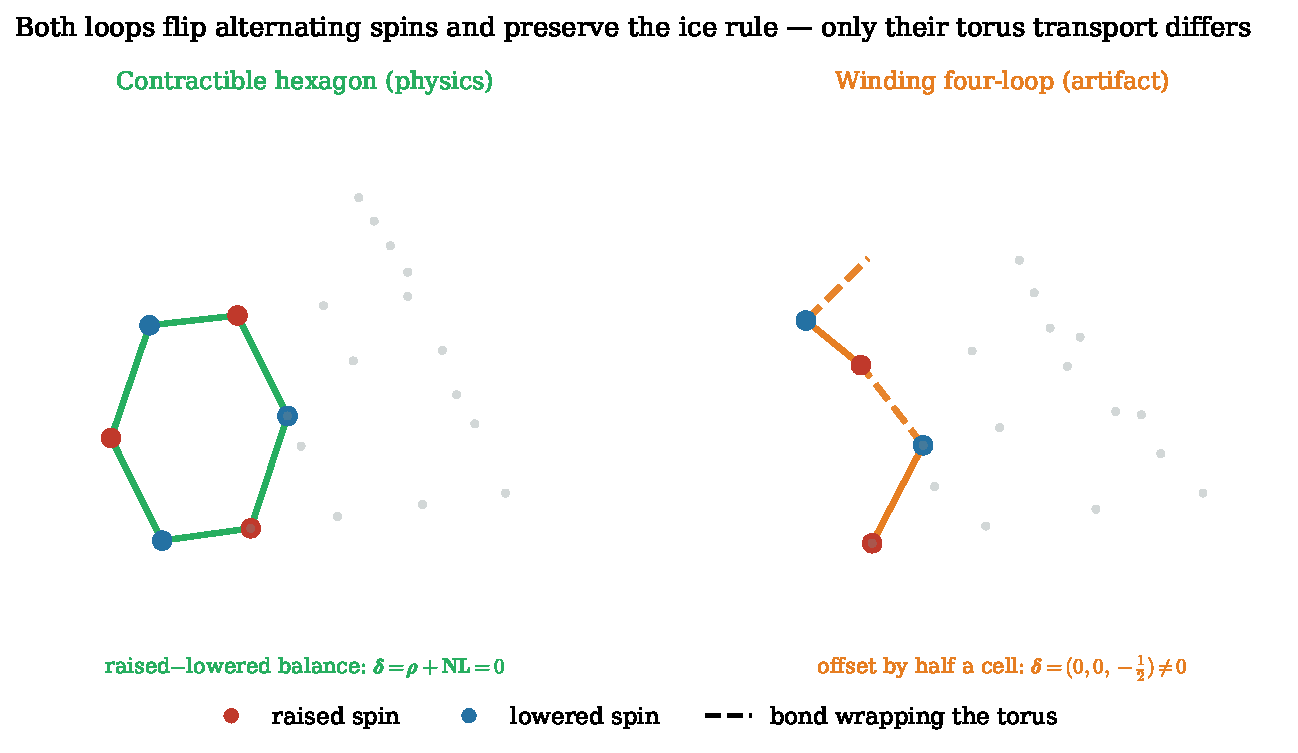
\includegraphics[width=0.95\textwidth]{fig_real_loops.pdf}
\caption{\textbf{The transported dipole tells the two loops apart, on the
real $16$-site cubic cluster.}  Both loops flip alternating spins (red raised,
blue lowered) and both return the system to the ice manifold.  \emph{Left:}
the contractible hexagon is balanced---the raised and lowered spins average to
the same point---so its transported dipole vanishes,
$\bdelta=\brho+\bN\bL=0$.  \emph{Right:} the winding four-loop must cross the
torus wall (dashed bonds); its raised and lowered spins are offset by half a
unit cell, giving $\bdelta=(0,0,-\tfrac12)\neq0$.  Selecting $\bdelta=0$ keeps
the left process and discards the right one.}
\label{fig:real_loops}
\end{figure}

\begin{lemma}[Gauge invariance of $\bdelta$]
The vector $\bdelta_r$ is independent of the choice of home cell and of the
gauge used to place the twist phases.
\end{lemma}

\begin{proof}
Move a site coordinate by a cluster translation, $\br_i\mapsto
\br_i+\bm m\bL$ with $\bm m\in\Z^3$.  If that site is raised, $\brho$
changes by $+\bm m\bL$; if it is lowered, $\brho$ changes by
$-\bm m\bL$.  The image bookkeeping of the virtual path changes by the
opposite integer vector, because the same physical hop is now represented
using a different periodic image.  Therefore $\bN\bL$ changes by the
negative of the change in $\brho$, and the sum $\brho+\bN\bL$ is unchanged.
\end{proof}

\begin{proposition}[Transported-dipole character projection]
For the clusters considered here, all coordinates lie on the quarter-lattice,
so every transported dipole has components in $\frac14\Z$.  We therefore define
the integer label
\begin{equation}
\boxed{\bDelta_r\equiv4\bdelta_r\in\Z^3.}
\label{eq:Delta_integer_label}
\end{equation}
This is only a change of units.  For example, the winding four-loop in
Fig.~\ref{fig:real_loops} has
$\bdelta=(0,0,-\tfrac12)$, hence $\bDelta=(0,0,-2)$.  The condition
$\bDelta=0$ is exactly the same condition as $\bdelta=0$.

Couple an auxiliary character field $\btheta$ to this integer transported
dipole.  A perturbative row $r$ acquires the phase
\begin{equation}
c_r(\btheta)=c_r e^{-i\btheta\cdot\bDelta_r}.
\label{eq:delta_character_phase}
\end{equation}
The operator-level average over $\btheta\in[0,2\pi)^3$ keeps exactly the rows
with $\bdelta_r=0$.
\end{proposition}

\begin{proof}
The characters of the abelian group $\Z^3$ are orthogonal:
\[
\overline{c_r}
=c_r\int_{[0,2\pi)^3}\frac{d^3\theta}{(2\pi)^3}
e^{-i\btheta\cdot\bDelta_r}
=c_r\,\delta_{\bDelta_r,0}.
\]
Since $\bDelta_r=4\bdelta_r$, the condition $\bDelta_r=0$ is equivalent to
$\bdelta_r=0$.
\end{proof}

\begin{remark}[How many discrete character points are needed?]
The exact integral over $\btheta$ can be replaced by a finite Fourier sum if
the grid separates the transported-dipole sectors present in the calculation.
For one component,
\[
\frac1M\sum_{m=0}^{M-1}
e^{-i(2\pi m/M)\Delta}
=
\begin{cases}
1,& \Delta=0\pmod M,\\
0,& \Delta\ne0\pmod M.
\end{cases}
\]
Thus the finite grid projects onto $\Delta=0$ only modulo $M$.  In the
order-$\Jpm^2$ and order-$\Jpm^3$ row data, the nonzero components of
$4\bdelta$ are $\pm2$.  Therefore the $4\bdelta$ convention needs a grid with
$M\nmid 2$; the smallest choice is $M=3$.  If instead one worked only at the
already-projected effective-row level and defined the integer label
$\widetilde{\bDelta}=2\bdelta$, then the nonzero components would be $\pm1$ and
an $M=2$ character average would distinguish them from zero.  We keep
$4\bdelta$ for the microscopic protocol because a single nearest-neighbor hop
can carry a quarter-lattice displacement, so $4\bd_{ij}$ is the natural integer
bond label.

This is a pure aliasing issue.  Consider one spurious four-loop component with
$\delta_\mu=-\frac12$.  With the effective-row label
$\widetilde\Delta_\mu=2\delta_\mu=-1$, the two-point average gives
\[
\frac12\left(1+e^{-i\pi(-1)}\right)=0,
\]
so the row is removed.  With the microscopic integer label
$\Delta_\mu=4\delta_\mu=-2$, the same two-point average gives
\[
\frac12\left(1+e^{-i\pi(-2)}\right)=1,
\]
so the row is not removed at all.  The nonzero sector has aliased back into the
zero sector modulo $2$.  The three-point average fixes this:
\[
\frac13\left(1+e^{-i(2\pi/3)(-2)}
 +e^{-i(4\pi/3)(-2)}\right)=0.
\]
The perturbative row-table check on the $16$-site cluster gives exactly this:
\[
\begin{array}{c|c|c}
\text{integer label} & M & \text{relative error to strict }\bdelta=0\\
\hline
4\bdelta & 2 & 11.6476\\
4\bdelta & 3 & 1.1\times10^{-15}\\
2\bdelta & 2 & 0\\
2\bdelta & 3 & 7.5\times10^{-16}
\end{array}
\]
Thus $M=2$ was never universally correct; it was correct only after choosing
the minimal effective-row charge $2\bdelta$.  Once the microscopic charge
$4\bdelta$ is used, $M=2$ aliases the artifact and $M=3$ is the smallest
correct grid for the order-$\Jpm^2$ and order-$\Jpm^3$ row data.
\end{remark}

\begin{remark}[Why physical twists were insufficient]
A physical flat vector potential gives phases of the form
$e^{-i\bA\cdot\bdelta_r}$.  On the $16$-site cluster the spurious four-loops
have half-cell transported dipoles, so the corresponding exponent is
half-integer in $2\pi$ units.  Physical twist averaging therefore suppresses
these rows but does not project them out exactly.  The auxiliary character
field in Eq.~\eqref{eq:delta_character_phase} is the finite-cluster source
conjugate to the integer transported dipole $\bDelta=4\bdelta$.
\end{remark}

\begin{corollary}[Clean ice-manifold Hamiltonian]
The artifact-free gauge Hamiltonian is
\begin{equation}
\boxed{
\Hclean(\Jpm)=
\sum_{r:\,\bdelta_r=0} c_r\Jpm^{k_r}|t_r\rangle\langle s_r| .
}
\label{eq:hclean}
\end{equation}
It keeps contractible hexagons and removes winding four-loops and wrapping
hexagons.
\end{corollary}

\section{Why the projection must act on the Hamiltonian}
\label{sec:operator-level}

The specific heat is nonlinear in the spectrum, and the spectrum is a
nonlinear function of the Hamiltonian.  Therefore
\begin{equation}
C\!\left[T;\frac1{N_\phi}\sum_\phi H(\phi)\right]
\ne
\frac1{N_\phi}\sum_\phi C[T;H(\phi)]
\end{equation}
in general.  Averaging observables after diagonalization can leave positive
even-in-coupling effects from a spurious matrix element.  The projection
must be applied at the operator level:
\begin{equation}
\Heff \longrightarrow \Hclean
\quad\text{first, then diagonalize.}
\end{equation}

\section{Practical algorithm}

For a production ED calculation in the gauge sector:
\begin{enumerate}
\item Build the periodic pyrochlore cluster.  Store each nearest-neighbor
bond $(i,j)$ and its image vector $\bn_{ij}$.
\item Enumerate tetrahedra and the ice manifold $\ice$.
\item Construct path-resolved Schrieffer--Wolff row tables
$H_2,H_3,H_4,\ldots$ at $\Jpm=1$.
\item For every row, compute $\brho$, $\bN$, and
$\bdelta=\brho+\bN\bL$.
\item Assemble either the bare matrix
\[
\Heff^{\mathrm{bare}}(\Jpm)=
\sum_r c_r\Jpm^{k_r}|t_r\rangle\langle s_r|
\]
or the clean matrix in Eq.~\eqref{eq:hclean}.
\item Diagonalize the ice-manifold matrix.  The $2\times2\times2$ FCC
cluster has only 2970 ice states, so dense diagonalization is exact and
cheap.
\item Compute $C(T)$, entropy, and low-energy $S^{zz}(\bq,\omega)$ from the
clean eigenstates.
\end{enumerate}

\section{The campaign: a holonomy-resolved microscopic ED protocol}

The effective-Hamiltonian calculation gives the target: the clean gauge
sector is the contractible-hexagon manifold.  The real ED campaign is to
obtain the same object without first expanding the Hamiltonian by hand.  The
microscopic protocol should take the full Hamiltonian, diagonalize its
low-energy ice-like band, and then remove precisely the components whose only
reason for existing is torus winding.  The organizing principle is not a
numerical counterterm; it is the topology of a compact $U(1)$ gauge theory on
a three-torus.

\subsection{Gauge-theory interpretation of the ice manifold}

The pyrochlore lattice is the line graph of the diamond lattice.  A spin on a
pyrochlore site is naturally a directed electric field on a diamond link
$\ell=(rr')$:
\begin{equation}
E_{\ell}=S^z_i
\end{equation}
up to a fixed convention for the link orientation.  The ice rule is Gauss'
law,
\begin{equation}
(\nabla\cdot E)_r=\sum_{\ell\supset r}\eta_{r\ell}E_\ell=0.
\label{eq:gauss_law}
\end{equation}
Thus the ice manifold is the zero-charge sector of a compact lattice gauge
theory.  The transverse exchange is the microscopic quantum dynamics that,
after virtual spinon fluctuations are integrated out, generates magnetic
terms of the form
\begin{equation}
\Heff^{\mathrm{bulk}}
=-g_{\mathrm{hex}}\sum_{p\in\mathrm{hexagons}}
\cos\!\left[(\nabla\times A)_p\right]+\cdots .
\label{eq:gauge_ring}
\end{equation}
Here $A_\ell$ is the compact vector potential conjugate to $E_\ell$.
Equation~\eqref{eq:gauge_ring} is local: each plaquette $p$ is a
contractible diamond hexagon.  Local magnetic dynamics cannot know about a
global torus cycle.

On a torus there are also harmonic, topological data.  Define electric fluxes
through the three noncontractible cuts,
\begin{equation}
W_\mu=\sum_{\ell\in\Sigma_\mu} E_\ell,\qquad \mu=x,y,z.
\label{eq:electric_flux}
\end{equation}
Contractible hexagon flips preserve $\bW=(W_x,W_y,W_z)$ exactly.  A loop
that winds around the torus is different: it carries a nontrivial homology
class in
\begin{equation}
H_1(T^3,\Z)=\Z^3 .
\end{equation}
Such a process is a Wilson line around a noncontractible cycle, not a local
plaquette.  In the thermodynamic gauge theory it is a finite-size tunnelling
event between global sectors, and its amplitude should vanish exponentially
with linear size.  In a tiny periodic cluster, however, the same
noncontractible path can be only four sites long, so it appears at the wrong
power of $\Jpm$.

\begin{intuition}
The physical photon comes from small magnetic curls: contractible hexagons.
The artifact comes from a Wilson loop that wraps around the whole torus but
looks short because the torus is too small.  The two processes can flip the
same number of spins locally, but they live in different topology classes.
\end{intuition}

\subsection{From flat holonomy to transported-dipole characters}

Threading a physical twist through the periodic cluster is the same as
coupling the spins to a flat background gauge field.  A flat connection has
zero local magnetic field but nontrivial holonomies
\begin{equation}
\Phi_\mu=\oint_{\gamma_\mu} \bA\cdot d\br=\phi_\mu
\end{equation}
around the three fundamental torus cycles.  A contractible process sees no
net holonomy.  A process with winding vector $\bw\in\Z^3$ picks up the
character
\begin{equation}
\chi_{\bw}(\bphi)=e^{-i\bw\cdot\bphi}.
\label{eq:holonomy_character}
\end{equation}
This is the correct language for integer homology.  The finite-size loops
found above are slightly subtler.  On the $16$-site cubic cluster their
transported dipoles are half-cell displacements: in the integer coordinates
\begin{equation}
\bDelta_r\equiv4\bdelta_r
\label{eq:delta4_def}
\end{equation}
the offending rows have components $\Delta_\mu=0,\pm2$, whereas the clean
hexagons have $\bDelta=0$.  An ordinary $2\pi$-periodic flat holonomy is not
orthogonal to a half-integer displacement.  This is why physical twist
averaging suppresses the artifact but does not reproduce the strict
$\bdelta=0$ projector.

The factor $4$ has no independent physical content.  It is the denominator of
the coordinate grid used for the pyrochlore sites.  The exact projector needs a
compact character variable with $2\pi$ periodicity:
\[
\int_0^{2\pi}\frac{d\theta}{2\pi}e^{-i\theta n}=\delta_{n,0}
\qquad (n\in\Z).
\]
If we used the real displacement $\delta_\mu=-\tfrac12$ directly, the exponent
$e^{-i\theta\delta_\mu}$ would not be a single-valued character on the
$2\pi$-periodic $\theta$ circle.  Multiplying by $4$ converts all possible
finite-cluster transported dipoles into integer labels.  Since multiplication
by $4$ is invertible as a test of zero, it changes no physics in the
projection: $\bDelta=0$ if and only if $\bdelta=0$.

The exact character variable for the finite cluster is therefore not the
integer winding $\bw$, but the integer transported dipole $\bDelta=4\bdelta$:
\begin{equation}
\chi_{\bDelta}(\btheta)=e^{-i\btheta\cdot\bDelta},
\qquad \bDelta\in\Z^3.
\label{eq:delta_character}
\end{equation}
Equivalently, the effective-Hamiltonian rows decompose into Fourier
characters of $\bDelta$:
\begin{equation}
\Heff(\btheta)=
\sum_{\bDelta\in\Z^3}{\Heff}_{\bDelta}\,
e^{-i\btheta\cdot\bDelta}.
\label{eq:delta_character_decomposition}
\end{equation}
The clean local gauge Hamiltonian is the trivial transported-dipole
character:
\begin{equation}
{\Heff}_{\mathrm{local}}={\Heff}_{\bDelta=0}
=\int_{[0,2\pi)^3}\frac{d^3\theta}{(2\pi)^3}\,\Heff(\btheta).
\label{eq:trivial_delta_character_projection}
\end{equation}
The important word is still \emph{operator}.  Equation~\eqref{eq:trivial_delta_character_projection}
is not an average of spectra.  It is a projection in the group algebra of
transported-dipole characters.

\begin{proposition}[Transported-dipole character projection]
Assume the low-energy ice-band operator admits the decomposition
Eq.~\eqref{eq:delta_character_decomposition}.  Averaging the operator over
the character field $\btheta$ keeps exactly the zero-transport component and
removes all nonzero transported dipoles:
\[
\int\frac{d^3\theta}{(2\pi)^3}\,\Heff(\btheta)={\Heff}_{\bDelta=0}.
\]
\end{proposition}

\begin{proof}
The characters $e^{-i\bDelta\cdot\btheta}$ are orthonormal on the
three-torus:
\[
\int\frac{d^3\theta}{(2\pi)^3}e^{-i(\bDelta-\bDelta')\cdot\btheta}
=\delta_{\bDelta,\bDelta'}.
\]
Applying this identity to Eq.~\eqref{eq:delta_character_decomposition}
selects the coefficient with $\bDelta=0$.  Contractible hexagons have
$\bDelta=0$; wrapping finite-size loops have $\bDelta\ne0$.
\end{proof}

\subsection{Pulling the microscopic low band back to the ice basis}

For the full microscopic Hamiltonian, the virtual paths are not explicitly
enumerated.  Instead we expose their transported dipole by diagonalizing a
character-deformed Hamiltonian.  For a nearest-neighbor bond represented by
the minimum-image displacement
\[
\bd_{ij}=\br_j-\br_i-\bn_{ij}\bL,
\]
the microscopic move $S_i^+S_j^-$ raises site $i$ and lowers site $j$, so its
transported-dipole increment is $-\bd_{ij}$.  The deformation whose virtual
paths acquire the character $e^{-i\btheta\cdot\bDelta}$ is therefore
\begin{equation}
\Hmic^{\Delta}(\btheta)=
\Jzz\sum_{\langle ij\rangle}S_i^zS_j^z
-\Jpm\sum_{\langle ij\rangle}
\left[
e^{+i\btheta\cdot(4\bd_{ij})}S_i^+S_j^-
+e^{-i\btheta\cdot(4\bd_{ij})}S_i^-S_j^+
\right],
\label{eq:mic_dipole_twisted}
\end{equation}
where $4\bd_{ij}$ is an integer vector on the clusters considered here.  This
is not an ordinary physical flux insertion.  It is an auxiliary source field
conjugate to the finite-cluster transported dipole.  Physical flat twists are
still useful diagnostics, but Eq.~\eqref{eq:mic_dipole_twisted} is the
deformation that reduces to the exact $\bdelta=0$ projection in perturbation
theory.

Let $\{|\psi_n(\btheta)\rangle\}_{n=1}^{N_{\ice}}$ be the lowest ice-like band
of $\Hmic^{\Delta}(\btheta)$, with energies $E_n(\btheta)$.  Let
\[
P_{\ice}=\sum_{\alpha\in\ice}|\alpha\rangle\langle\alpha|
\]
be the projector onto the fixed classical ice basis.  Define the projected
band matrix
\begin{equation}
X_{\alpha n}(\btheta)=\langle\alpha|\psi_n(\btheta)\rangle .
\end{equation}
If the microscopic low band is really the dressed ice manifold, then
\begin{equation}
G(\btheta)=X^\dagger(\btheta)X(\btheta)
\end{equation}
is nonsingular and close to the identity.  The Loewdin-orthonormalized pullback
is
\begin{equation}
Q(\btheta)=X(\btheta)\,G^{-1/2}(\btheta),
\qquad Q^\dagger Q=1.
\label{eq:lowdin_pullback}
\end{equation}
The full-Hamiltonian band operator, represented in one fixed ice basis, is
\begin{equation}
\HB(\btheta)=
Q(\btheta)\,\mathrm{diag}\{E_n(\btheta)\}\,Q^\dagger(\btheta).
\label{eq:band_operator}
\end{equation}
This is the object to filter.  It contains all orders in $\Jpm/\Jzz$ that are
present in the microscopic ED data, but it is expressed on the same ice
manifold on which the gauge theory acts.

\subsection{The clean microscopic operator}

The proposed microscopic artifact-removal prescription is
\begin{equation}
\boxed{
{\HB}^{\mathrm{clean}}
=\int_{[0,2\pi)^3}\frac{d^3\theta}{(2\pi)^3}\,\HB(\btheta).
}
\label{eq:clean_band_operator}
\end{equation}
Equation~\eqref{eq:clean_band_operator} is the full-Hamiltonian analogue of
Eq.~\eqref{eq:hclean}.  In the perturbative limit it reduces to the
$\bdelta=0$ row projection.  Away from the strict perturbative limit it is
still meaningful: it extracts the component of the dressed ice band that is
neutral under all transported-dipole characters.

For numerical work the integral is replaced by a Fourier quadrature,
\begin{equation}
{\HB}^{(0)}_{M}=
\frac{1}{M^3}\sum_{m_x,m_y,m_z=0}^{M-1}
\HB\!\left(\frac{2\pi m_x}{M},
           \frac{2\pi m_y}{M},
           \frac{2\pi m_z}{M}\right),
\qquad \HB=\HB(\btheta).
\label{eq:grid_projection}
\end{equation}
For the $16$-site campaign below we use the minimal effective-row label
\[
\widetilde{\bDelta}=2\bdelta .
\]
The spurious four-loop sectors then carry $\widetilde\Delta_\mu=\pm1$, so the
two-point grid $M=2$ distinguishes them from zero.  This is the smallest
character average that exactly reproduces the strict $\bdelta=0$ row projector
through order $\Jpm^3$.  With the alternative microscopic integer label
$\bDelta=4\bdelta$, the same artifacts carry $\Delta_\mu=\pm2$, so $M=2$
aliases them back to zero and one needs $M=3$.

In larger clusters or at higher perturbative order, $M$ should be increased
until $C(T)$, the low-band spectrum, and selected matrix elements of
${\HB}^{(0)}_M$ converge.

\subsection{Concrete ED protocol}

The full microscopic calculation should therefore be organized as follows.
\begin{enumerate}
\item Choose a periodic cluster and construct a fixed ice basis
$\{|\alpha\rangle\}$.
\item For each character field $\btheta$ on the grid, build the source-deformed
microscopic Hamiltonian in the full fixed-$S^z_{\rm tot}=0$ Hilbert space.  In
the adopted $2\bdelta$ protocol, replace $4\bd_{ij}$ by $2\bd_{ij}$ in
Eq.~\eqref{eq:mic_dipole_twisted} and use the $M=2$ grid
$\theta_\mu\in\{0,\pi\}$.
\item Diagonalize the lowest $N_{\ice}$ states.  Record the spectral
separation between the $N_{\ice}$th and $(N_{\ice}+1)$st levels whenever
possible.
\item Project the eigenvectors onto the ice basis and monitor
\[
\lambda_{\min}\!\left[X^\dagger(\btheta)X(\btheta)\right].
\]
If this value is too small, the chosen coupling is outside the regime where a
clean ice-band pullback is controlled.
\item Construct $\HB(\btheta)$ using Eq.~\eqref{eq:band_operator}.
\item Perform the operator-level character projection
Eq.~\eqref{eq:grid_projection}.  Diagonalize only after this step.
\item Validate the method by the weak-coupling limit:
\[
{\HB}^{(0)}_M-\text{const.}
=\Hclean+O(\Jpm^4/\Jzz^3)
\]
when $M$ resolves the winding characters present through third order.
\item Use the resulting eigenstates for the low-temperature gauge-sector
thermodynamics and for observables such as $S^{zz}(\bq,\omega)$ that do not
leave the ice manifold.
\end{enumerate}

\subsection{First microscopic test on the 16-site cluster}

We performed this test with the local QED package on the $16$-site cubic
cluster at $\Jpm=-0.05\Jzz$.  The full fixed-$S^z_{\rm tot}=0$ Hilbert space
has dimension
\[
\binom{16}{8}=12870,
\]
and the ice band has $N_{\ice}=90$ states.  Dense partial diagonalization was
used to obtain the lowest $90$ eigenvectors at each source-field point.

The perturbative row-table test first establishes the correct source field.
On this cluster, physical flat twists and integer winding projectors do not
match the strict $\bdelta=0$ Hamiltonian.  The transported-dipole character
does:
\begin{center}
\footnotesize
\begin{tabular}{@{}p{0.30\linewidth}p{0.14\linewidth}p{0.20\linewidth}p{0.22\linewidth}@{}}
\toprule
projector & $T_{\rm peak}/\Jzz$ & rel. error to $\bdelta=0$
& comment\\
\midrule
all rows & $0.0100564$ & $11.6476$ & winding four-loop present\\
integer $N=0$ & $0.0046462$ & $5.8238$ & boundary winding only\\
physical $\bA\!\cdot\!\bdelta$, $M=6$ & $0.0016563$ & $3.0740$
& suppresses, not exact\\
$2\bdelta$ character, $M=2$ & $0.0016045$ & $0$
& minimal row-level charge\\
$\bDelta=4\bdelta$ character, $M=3$ & $0.0016045$ & $0$
& exact through order $3$\\
\bottomrule
\end{tabular}
\end{center}

We tested both microscopic source conventions.  The adopted $2\bdelta$ run used
Eq.~\eqref{eq:mic_dipole_twisted} with $4\bd_{ij}$ replaced by $2\bd_{ij}$ on
the $M=2$ grid, i.e. $8$ source-field points.  The $\bDelta=4\bdelta$ comparison
run used Eq.~\eqref{eq:mic_dipole_twisted} on the $M=3$ grid, i.e. $27$
source-field points.  The low-band pullback was well conditioned in both cases;
for the $2\bdelta$ run,
\[
\min_{\btheta}\lambda_{\min}\!\left[
X^\dagger(\btheta)X(\btheta)\right]
=0.8872896692,
\]
and the QED eigenvectors were orthonormal to $2.3\times10^{-14}$.
The resulting specific-heat peaks are
\begin{center}
\begin{tabular}{lcc}
\toprule
operator & $T_{\rm peak}/\Jzz$ & comment\\
\midrule
full QED band, $\btheta=0$ & $0.0129476$ & matches all-row physics\\
full QED band, $2\bdelta$ character $M=2$ & $0.0012227$
& near clean scale, not identical\\
full QED band, $4\bdelta$ character $M=3$ & $0.0012222$
& better operator match\\
perturbative all rows & $0.0100564$ & four-loop artifact\\
perturbative $\bdelta=0$ & $0.0016045$ & clean hexagon target\\
\bottomrule
\end{tabular}
\end{center}

The equality claim in the perturbative table is an operator statement inside
the order-$\Jpm^2$ and order-$\Jpm^3$ ice-manifold row table.  It does not imply
that the finite-$\Jpm$ full-Hamiltonian specific heat peak must land exactly at
the perturbative $\bdelta=0$ peak.  The full QED low band contains
Schrieffer-Wolff dressing and higher-order terms beyond the truncated row
table, and the specific heat is a nonlinear function of the final projected
spectrum.  The appropriate full-Hamiltonian check is therefore whether the
character projection removes the four-loop-scale peak and moves the result to
the clean hexagon scale, not whether the peak positions are numerically
identical at $\Jpm=-0.05\Jzz$.

\begin{figure}[htbp]
\centering
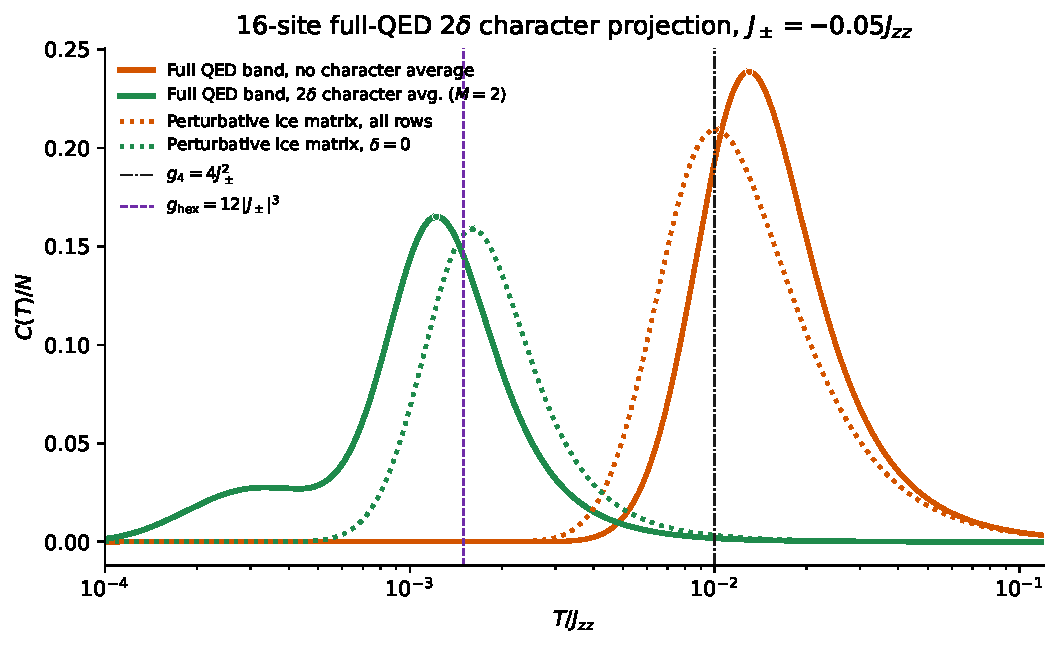
\includegraphics[width=0.78\textwidth]{fig_qed_dipole2_M2_specific_heat.pdf}
\caption{\textbf{Specific heat from the adopted $2\bdelta$, $M=2$ full-QED
protocol.}  The orange solid curve is the untwisted full microscopic low-band
pullback.  The green solid curve is the operator-level $2\bdelta$ character
average over the $M=2$ grid.  Dotted curves are the perturbative ice-manifold
matrices with all rows and with the strict $\bdelta=0$ projector.  The character
average moves the low-temperature peak from the spurious four-loop scale toward
the clean hexagon scale.}
\label{fig:qed_dipole2_m2_specific_heat}
\end{figure}

At the operator level, after removing constants, the adopted $2\bdelta$, $M=2$
projected full QED band has relative Frobenius error $0.3527$ against the
perturbative $\bdelta=0$ matrix.  Allowing one overall scale factor, the
residual falls to $0.2612$; the corresponding spectrum residual is also
$0.2612$.  The $4\bdelta$, $M=3$ comparison run gives a slightly better
operator residual, $0.1450$ after scale fitting, but it requires $27$ full ED
points instead of $8$.  Thus the working protocol for the present $16$-site
campaign is the cheaper and perturbatively minimal $2\bdelta$, $M=2$ character
average.  Both character protocols are a large improvement over the ordinary
physical $M=2$ holonomy average, whose operator error against $\bdelta=0$ was
$5.4308$.

Thus the first microscopic test supports the corrected campaign: full ED
dresses the ice manifold, while the transported-dipole character projection
removes the dominant finite-size four-loop and recovers the clean hexagon
scale up to higher-order dressing of the microscopic band.

\end{document}
